\section{DLB version analysis}

In Figure \ref{fig:plot-hybrid-dlb-int}, we compare the integration time between the hybrid version and the DLB version on the configurations we tested in the previous section. This time, we don't check all grainsize values. Instead, we choose the ideal for each input. We can observe that applying DLB makes all configurations faster than the pure MPI version and all the hybrid configurations. It is also remarkable that there is no notable difference between hybrid configurations. On the detailed chemistry (Figure \ref{fig:plot-hybrid-dlb-int-det}) we see that with DLB we achieve a \textit{x2} respect the original. On the reduced chemistry (Figure \ref{fig:plot-hybrid-dlb-int-red}) we achieve a \textit{x7} with DLB on the best configuration (\textit{12x4}). Nonetheless, with the \textit{48x1} configuration, we achieve a \textit{x5} speedup against original.
\begin{figure}[ht]
  \begin{subfigure}{1\textwidth}
    \centering
    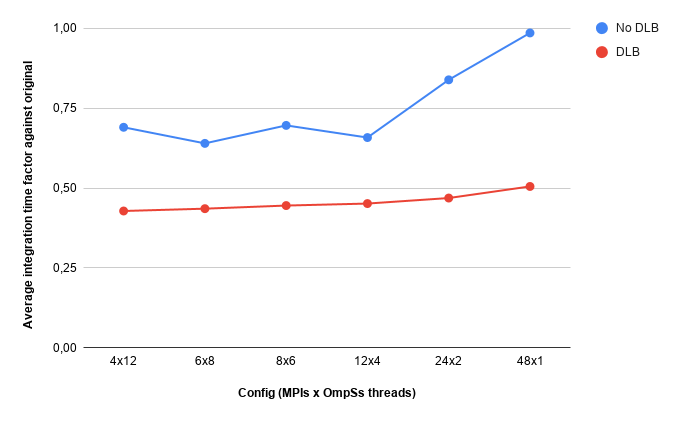
\includegraphics[width=0.7\textwidth]{graphics/hybridcompletedlb.png}
    \subcaption{Detailed chemistry case}
    \label{fig:plot-hybrid-dlb-int-det}

  \end{subfigure}
  \begin{subfigure}{1\textwidth}
    \centering
    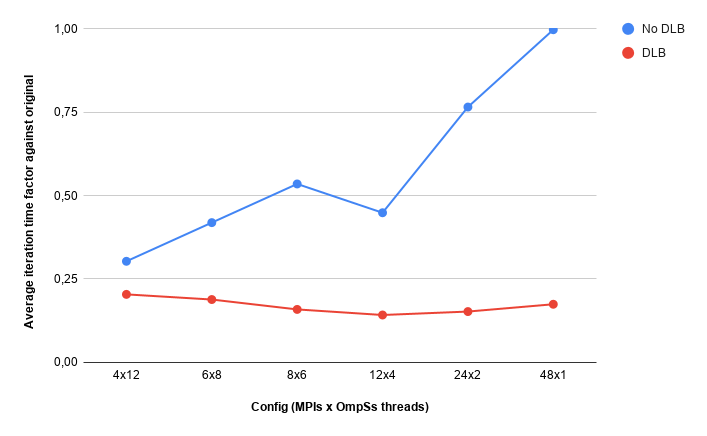
\includegraphics[width=0.7\textwidth]{graphics/hybridreduceddlb.png}
    \subcaption{Reduced chemistry case}
    \label{fig:plot-hybrid-dlb-int-red}

  \end{subfigure}

  \caption[DLB chemical integration time factor on hybrid configurations.]{DLB chemical integration time factor on hybrid configurations. Own compilation.}
  \label{fig:plot-hybrid-dlb-int}
\end{figure}

To see the overall performance, in Figure \ref{fig:plot-hybrid-dlb-it} we compare the average time step with and without DLB on the hybrid configurations with the ideal grainsize. As seen in the previous section, the hybrid configurations are far from the pure MPI version since the application is not fully parallelized with OmpSs. Although, in general terms with the \textit{48x1} configuration, we achieve a speedup in both inputs. On the detailed chemistry case (Figure \ref{fig:plot-hybrid-dlb-it-det}), we earn a \textit{1.5x} speedup. On the reduced chemistry case (Figure \ref{fig:plot-hybrid-dlb-it-red}), as the integration weight is lower, the speedup achieved is \textit{1.3x}.

\begin{figure}[ht]
  \begin{subfigure}{1\textwidth}
    \centering
    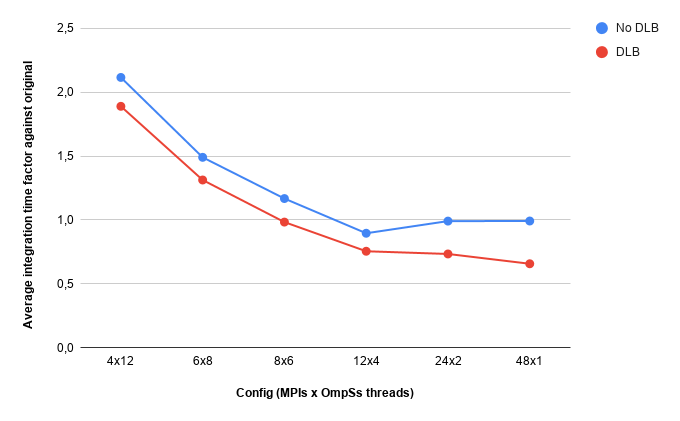
\includegraphics[width=0.7\textwidth]{graphics/hybridcompletedlbabs.png}
    \subcaption{Detailed chemistry case}
    \label{fig:plot-hybrid-dlb-it-det}

  \end{subfigure}
  \begin{subfigure}{1\textwidth}
    \centering
    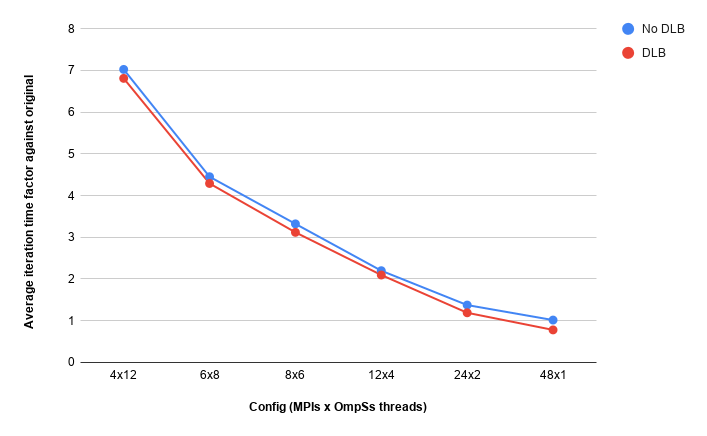
\includegraphics[width=0.7\textwidth]{graphics/hybridreduceddlbabs.png}
    \subcaption{Reduced chemistry case}
    \label{fig:plot-hybrid-dlb-it-red}

  \end{subfigure}

  \caption[DLB iteraiton time factor on hybrid configurations.]{DLB iteration time factor on hybrid configurations. Own compilation.}
  \label{fig:plot-hybrid-dlb-it}
\end{figure}

Now we will check how the optimization behaves when running with multiple nodes. Figure \ref{fig:plot-hybrid-dlb-int-mul} shows the integration time factor running with DLB against the pure MPI version with the same number of processes, both inputs, grainsize 16 for the complete integration and grainsize 32 for the reduced. We can see that in the complete integration case (Figure \ref{fig:plot-hybrid-dlb-int-mul-det}), the speedup is constant to \textit{2x}. On the reduced (Figure \ref{fig:plot-hybrid-dlb-int-mul-red}), DLB effectiveness is lost when increasing the number of nodes. This loss is probably because when we increase the number of nodes, the balance among nodes is worse. DLB can balance the workload difference within a node because it relays on a shared memory programming model. % In the next section, we will identify the problem using a DLB module and handle the issue.

\begin{figure}[ht]
  \begin{subfigure}{1\textwidth}
    \centering
    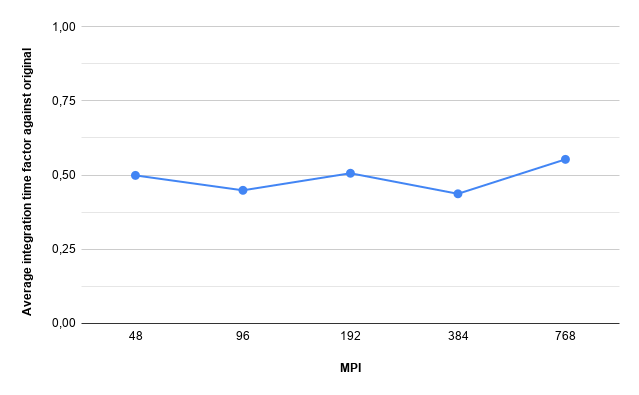
\includegraphics[width=0.7\textwidth]{graphics/hybridcompletedlbmulti.png}
    \subcaption{Detailed chemistry case}
    \label{fig:plot-hybrid-dlb-int-mul-det}

  \end{subfigure}
\begin{subfigure}{1\textwidth}
    \centering
    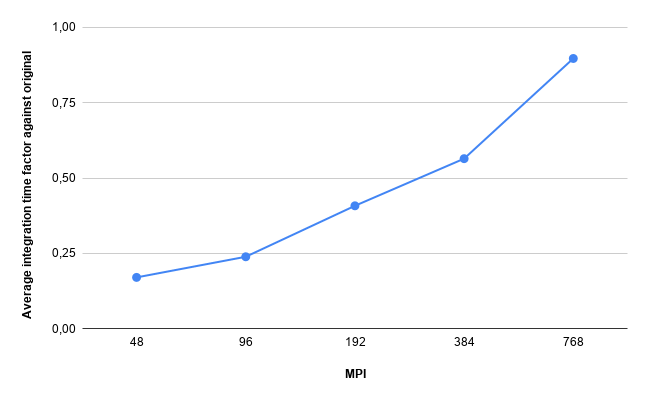
\includegraphics[width=0.7\textwidth]{graphics/hybridreduceddlbmulti.png}
    \subcaption{Reduced chemistry case}
    \label{fig:plot-hybrid-dlb-int-mul-red}

  \end{subfigure}

  \caption[DLB Chemical Integration time factor multinode.]{DLB Chemical Integration time factor multinode. Own compilation.}
  \label{fig:plot-hybrid-dlb-int-mul}
\end{figure}

Figure \ref{fig:plot-hybrid-dlb-int-mul-scal} presents the scalability plots of the same runs, with and without DLB. On the detailed case (Figure \ref{fig:plot-hybrid-dlb-int-mul-scal-det}), we see scalability from both versions are similar. This fact makes sense since the speedup showed in the last plot is constant, the scalability between the versions is analogous. On the reduced chemistry (Figure \ref{fig:plot-hybrid-dlb-int-mul-scal-red}) we observe that the DLB version's scalability is poor because as said, DLB loses effectiveness when increasing the number of processes.

\begin{figure}[ht]
  \begin{subfigure}{1\textwidth}
    \centering
    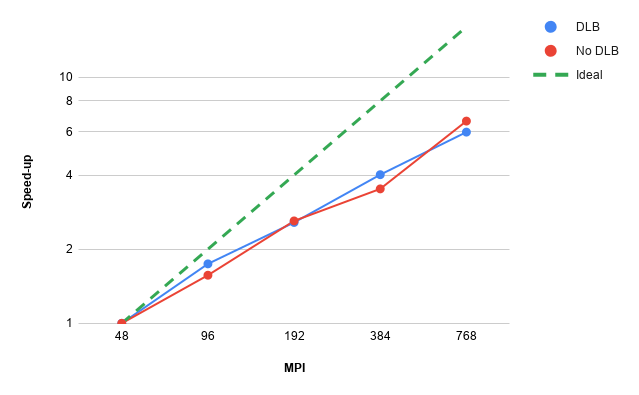
\includegraphics[width=0.7\textwidth]{graphics/hybridcompletedlbmultiscal.png}
    \subcaption{Detailed chemistry case}
    \label{fig:plot-hybrid-dlb-int-mul-scal-det}

  \end{subfigure}
  \begin{subfigure}{1\textwidth}
    \centering
    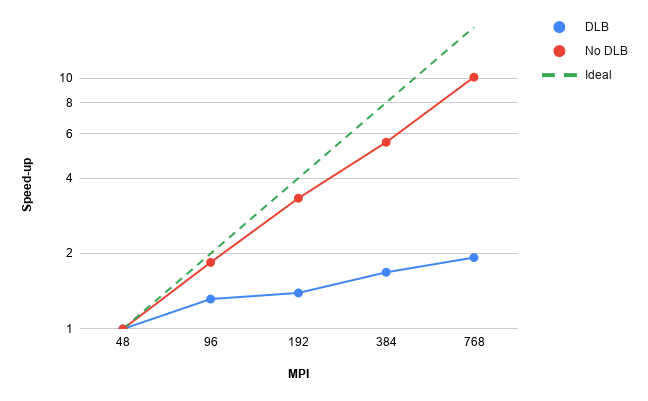
\includegraphics[width=0.7\textwidth]{graphics/hybridreduceddlbmultiscal.png}
    \subcaption{Reduced chemistry case}
    \label{fig:plot-hybrid-dlb-int-mul-scal-red}

  \end{subfigure}

  \caption[Chemical integration scalability comparison]{Chemical integration scalability comparison. Own compilation.}
  \label{fig:plot-hybrid-dlb-int-mul-scal}
\end{figure}
